\documentclass[13.5pt]{beamer}
\usepackage[natbib=true,backend=bibtex,useprefix=true]{biblatex}
\usepackage[utf8]{inputenc}
\usepackage{tikz}
\usepackage{ragged2e}
\usepackage{adjustbox}
\usepackage{amsmath}
\usepackage{amsfonts}
\usepackage{amssymb}
\usepackage{amsthm}
\usetikzlibrary{fadings}
\usepackage{fontspec}
\usepackage{unicode-math}
\setmathfont{XITS Math}
\usepackage{float}
\usepackage[caption = false]{subfig}
\usepackage{graphicx}



\usetheme{Madrid}

\definecolor{TorVergataColor}{RGB}{0,125,52}
\setsansfont[BoldFont={Circe-Bold}]{Circe-Regular}

\newcommand{\B}[1]{\textcolor{TorVergataColor}{\textbf{#1}}}
\newcommand{\Cross}{\mathbin{\tikz [x=2.5ex,y=2.5ex,line width=.10ex] \draw (0,0) -- (1,1) (0,1) -- (1,0);}}
\newcommand{\mathDef}{\overset{\textit{def}}{=}}
\newcommand{\N}{\mathbb{N}}
\newcommand{\R}{\mathbb{R}}
\newcommand{\Rplus}{\mathbb{R}^+}

\makeatletter
\setbeamertemplate{title page}{%
	\vbox{}
	\vfill
	{\usebeamercolor[fg]{titlegraphic}\inserttitlegraphic\par}
	\begingroup
	\centering
	\begin{beamercolorbox}[sep=8pt,center]{title}
		\usebeamerfont{title}\inserttitle\par%
		\ifx\insertsubtitle\@empty%
		\else%
		\vskip0.25em%
		{\usebeamerfont{subtitle}\usebeamercolor[fg]{subtitle}\insertsubtitle\par}%
		\fi%     
	\end{beamercolorbox}%
	\vskip1em\par
	\vfill%<- added
	\begin{beamercolorbox}[sep=8pt,left]{author}
		\usebeamerfont{author}\insertauthor
	\end{beamercolorbox}
	\vfill%<- added
	\begin{beamercolorbox}[sep=8pt,center]{institute}
		\usebeamerfont{institute}\insertinstitute
	\end{beamercolorbox}
	\vfill%<- added
	\begin{beamercolorbox}[sep=8pt,center]{date}
		\usebeamerfont{date}\insertdate
	\end{beamercolorbox}%
	\vskip0cm%<- changed
	%    
	\endgroup
	\vfill%<- removed
}
\makeatother



\setbeamercolor{structure}{fg=TorVergataColor}
\setbeamerfont{structure}{family=\bfseries,size=\large}

\title[]
{ 
	\textbf{A QoS-Aware Broker \\ for Multi-Provider Serverless Applications}
}

\author[Andrea Graziani (m. 0273395)]{{\Large \textbf{Andrea Graziani}}\\m. $0273395$\\[10mm]{\small 
		\begin{tabular}{l|l}
			\textbf{Supervisor}: & \textit{Valeria Cardellini } \\ 
			\textbf{Tutor}: & \textit{Gabriele Russo Russo}  \\  
\end{tabular}}}

\titlegraphic{
\includegraphics[width=9.5cm,height=2.4cm]{../Images/UniLogo/LogoMacroarea.png}}

\setbeamertemplate{background}{%
	\begin{tikzpicture}[overlay,remember picture]
		\node[scope fading=west,anchor=north west] at ([shift={(2in,-1in)}]current page.north west) {
\includegraphics[width=9cm,height=9cm]{../Images/UniLogo/TorVergataWatermark.png}};
	\end{tikzpicture}
}

\justifying

\setbeamertemplate{frametitle}{%
	\nointerlineskip%
	\begin{beamercolorbox}[wd=\paperwidth,ht=4.0ex,dp=1ex]{frametitle}
		\hspace*{1ex}\insertframetitle%
	\end{beamercolorbox}%
}

\addtobeamertemplate{frametitle}{}{%
	\begin{tikzpicture}[remember picture,overlay]
		\node[anchor=north east,yshift=2pt] at (current page.north east) {
\includegraphics[height=1cm]{../Images/UniLogo/NegativeTorVergataLogo.png}};
\end{tikzpicture}}

\date{May 23, 2022}

%-------------------------------------------------------
% THE BODY OF THE PRESENTATION
%-------------------------------------------------------




\begin{document}

%-------------------------------------------------------
% THE TITLEPAGE
%-------------------------------------------------------

{% % this is the name of the PDF file for the background
\begin{frame}[plain,noframenumbering] % the plain option removes the header from the title page, noframenumbering removes the numbering of this frame only
  \titlepage % call the title page information from above
\end{frame}}

\setbeamertemplate{background}{}

% -------------- %
% -------------- %
\begin{frame}{Serverless Computing: Overview}

\begin{block}{}
	\centering
	My thesis is focused on ``\B{serverless computing}".
\end{block}

\vspace{\baselineskip}
It is a development paradigm according to which:
\vspace{\baselineskip}
\begin{itemize}
	\justifying
	\item The provider takes care of all aspect of server management.
	\vspace{\baselineskip}
	\item Cloud application are abstracted as a group of so-called \\ \B{serverless functions}, which are computation units implementing a business functionality.

\end{itemize}

\end{frame} 
% -------------- %
% -------------- %
\begin{frame}{Serverless Computing: Overview}
	
	\begin{block}{}
		\centering
		A serverless function is executed inside a containerized environment: the so-called \B{function instance}.
	\end{block}

	\vspace{\baselineskip}
	
	\begin{block}{}
		\centering
		The FaaS platform \B{automatically} scales the number of function instances.
	\end{block}

	\vspace{\baselineskip}
	
	\begin{block}{}
		FaaS platforms impose a \B{limit} on the number of function instance runnable at the \B{same time} called \B{concurrency limit}.
	\end{block}

\vspace{\baselineskip}

\begin{block}{}
	A delay is observed when a new function instance is started by the provider: this event is called \B{cold start}.
\end{block}
		
\end{frame} 
% -------------- %
% -------------- %
\begin{frame}{Serverless Computing: Overview}
	
	\begin{block}{}
		To invoke a \B{serverless function}, users have to specify a so-called \B{serverless function configuration}.
		\begin{itemize}
			\item Generally, the \B{amount of memory allocated} to a serverless function.
		\end{itemize}
	\end{block}
	\vspace{\baselineskip}
	\begin{block}{}
		\centering
		Configuration parameters \B{significantly} affect the \B{cost} and \B{response time} of serverless functions.
	\end{block}
	
	
\end{frame} 
% -------------- %
% -------------- %
\begin{frame}{Serverless Computing: Problems}
	
	\begin{itemize}
		\item Lack of support for application whose functions are hosted on \B{multiple providers}.
		\vspace{\baselineskip}
		\item Lack of support for serverless function implementations abstraction, that is, for the so-called \B{concrete functions}.
		\vspace{\baselineskip}
		\item Fulfillment of \B{non-functional requirements} concerning the \B{quality of service} (QoS) levels that should be guaranteed for \B{multi-provider serverless applications}.
		\vspace{\baselineskip}
		\item Fulfillment of \B{functional requirements} concerning the \B{orchestration} of multi-provider applications.
	\end{itemize}

\end{frame} 
% -------------- %
% -------------- %

\begin{frame}{Thesis Goals}
	
	\begin{block}{Goal $\#$ 1}
		\centering
	To guarantee the \B{satisfaction of QoS levels} for multi-provider serverless applications. 
	\end{block}

	\vspace{\baselineskip}
	It was necessary to develop:
	\vspace{\baselineskip} 
	
	\begin{enumerate}
		\justifying
	
	\item An \B{analytical model} to evaluate aforementioned class of applications.

	\vspace{\baselineskip} 
	
	\item A \B{methodological way} to find the ``best" configuration to satisfy QoS constraints.
	
	\end{enumerate}
	\end{frame} 

% -------------- %
% -------------- %

\begin{frame}{Thesis Goals}
	
	\begin{block}{Goal $\#$ 2}
		\centering
		The \B{orchestration} for multi-provider serverless applications. 
	\end{block}
	
	\vspace{\baselineskip}
	To achieve it, I had to build:
	\vspace{\baselineskip}

	\begin{enumerate}
		\justifying
	
		\item A \B{software framework}.
		
		\vspace{\baselineskip} 
		\item An extension to an already existent \B{representation scheme} to define a serverless application workflow.
		\begin{itemize}
			\item Based on an existing language called \B{abstract function choreography language} (AFCL).
		\end{itemize}
		
	\end{enumerate}
	
\end{frame} 


% -------------- %
% -------------- %


% -------------- %
% -------------- %
\begin{frame}{System Model}
	
	\begin{block}{}
		\centering
		Serverless applications are abstracted to a \\\B{weakly connected weighted directed graph}.
	\end{block}
	\vspace{\baselineskip}
	\begin{Center}

	
	\resizebox{11cm}{5cm}{
		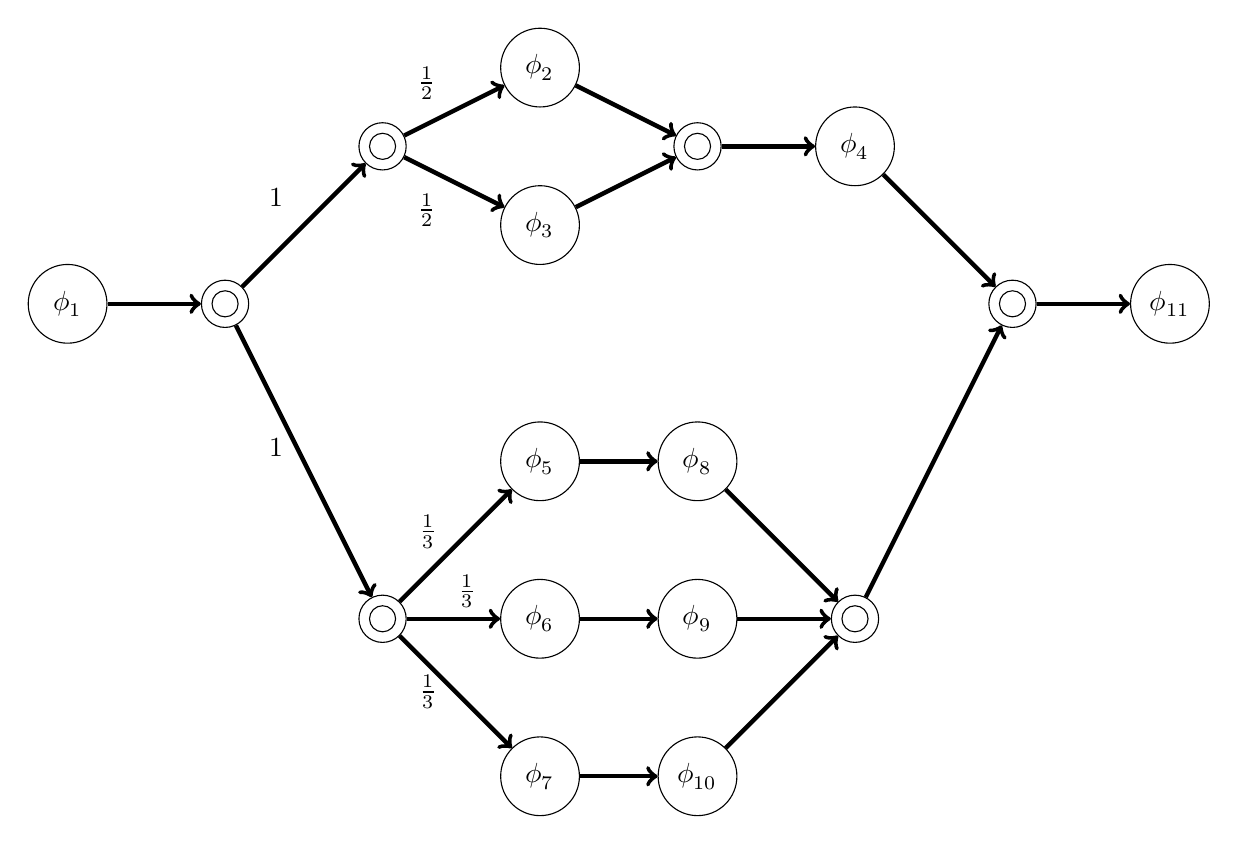
\begin{tikzpicture}
			
			
			\node[circle,draw,minimum width = 1cm] 
			(Func1) at (-2,0) {$\phi_1$};
			
			\node[circle, draw, minimum width = 0.2cm]        					   
			() at (0,0) {};
			\node[circle, draw, minimum width = 0.6cm]        					   
			(PAR-Enter) at (0,0) {};
			
			\draw[ultra thick,->] (Func1) -- (PAR-Enter);
			
			\node[circle, draw, minimum width = 0.2cm]        					   
			() at (2,2) {};
			\node[circle, draw, minimum width = 0.6cm]        					   
			(IF-Enter) at (2,2) {};
			
			\draw[ultra thick,->] (PAR-Enter) edge node[xshift=-10,yshift=10]{$1$} (IF-Enter);
			
			\node[circle, draw, minimum width = 1cm]       					   
			(Func2) at (4,3) {$\phi_2$};
			
			\draw[ultra thick,->] (IF-Enter) edge node[xshift=-10,yshift=10]{$\frac{1}{2}$} (Func2);
			
			\node[circle, draw, minimum width = 1cm]       					   
			(Func3) at (4,1) {$\phi_3$};
			
			\draw[ultra thick,->] (IF-Enter) edge node[xshift=-10,yshift=-10]{$\frac{1}{2}$} (Func3);
			
			\node[circle, draw, minimum width = 0.2cm]        					   
			() at (6,2) {};
			\node[circle, draw, minimum width = 0.6cm]        					   
			(IF-Exit) at (6,2) {};
			
			\draw[ultra thick,->] (Func2) edge node[xshift=-10,yshift=-10]{} (IF-Exit);
			\draw[ultra thick,->] (Func3) edge node[xshift=-10,yshift=-10]{} (IF-Exit);
			
			\node[circle, draw, minimum width = 1cm]       					   
			(Func4) at (8,2) {$\phi_4$};
			
			\draw[ultra thick,->] (IF-Exit) edge node[xshift=-10,yshift=-10]{} (Func4);
			
			\node[circle, draw, minimum width = 0.2cm]        					   
			() at (2,-4) {};
			\node[circle, draw, minimum width = 0.6cm]        					   
			(SWITCH-Enter) at (2,-4) {};
			
			\draw[ultra thick,->] (PAR-Enter) edge node[xshift=-10,yshift=5]{$1$} (SWITCH-Enter);
			
			\node[circle, draw, minimum width = 1cm]       					   
			(Func5) at (4,-2) {$\phi_5$};
			
			\draw[ultra thick,->] (SWITCH-Enter) edge node[xshift=-10,yshift=5]{$\frac{1}{3}$} (Func5);
			
			\node[circle, draw, minimum width = 1cm]       					   
			(Func6) at (4,-4) {$\phi_6$};
			
			\draw[ultra thick,->] (SWITCH-Enter) edge node[xshift=5,yshift=10]{$\frac{1}{3}$} (Func6);
			
			\node[circle, draw, minimum width = 1cm]       					   
			(Func7) at (4,-6) {$\phi_7$};
			
			\draw[ultra thick,->] (SWITCH-Enter) edge node[xshift=-10,yshift=0]{$\frac{1}{3}$} (Func7);
			
			\node[circle, draw, minimum width = 1cm]       					   
			(Func8) at (6,-2) {$\phi_8$};
			
			\draw[ultra thick,->] (Func5) edge node[xshift=-10,yshift=0]{} (Func8);
			
			\node[circle, draw, minimum width = 1cm]       					   
			(Func9) at (6,-4) {$\phi_9$};
			
			\draw[ultra thick,->] (Func6) edge node[xshift=-10,yshift=0]{} (Func9);
			
			\node[circle, draw, minimum width = 1cm]       					   
			(Func10) at (6,-6) {$\phi_{10}$};
			
			\draw[ultra thick,->] (Func7) edge node[xshift=-10,yshift=0]{} (Func10);
			
			\node[circle, draw, minimum width = 0.2cm]        					   
			() at (8,-4) {};
			\node[circle, draw, minimum width = 0.6cm]        					   
			(SWITCH-Exit) at (8,-4) {};
			
			\draw[ultra thick,->] (Func8) edge node[xshift=-10,yshift=0]{} (SWITCH-Exit);
			\draw[ultra thick,->] (Func9) edge node[xshift=-10,yshift=0]{} (SWITCH-Exit);
			\draw[ultra thick,->] (Func10) edge node[xshift=-10,yshift=0]{} (SWITCH-Exit);
			
			\node[circle, draw, minimum width = 0.2cm]        					   
			() at (10,0) {};
			\node[circle, draw, minimum width = 0.6cm]        					   
			(PAR-Exit) at (10,0) {};
			
			\draw[ultra thick,->] (SWITCH-Exit) edge node[xshift=-10,yshift=0]{} (PAR-Exit);
			\draw[ultra thick,->] (Func4) edge node[xshift=-10,yshift=0]{} (PAR-Exit);
			
			\node[circle,draw,minimum width = 1cm] 
			(Func11) at (12,0) {$\phi_{11}$};
			
			\draw[ultra thick,->] (PAR-Exit) edge node[xshift=-10,yshift=0]{} (Func11);
			
		\end{tikzpicture}
}
	\end{Center}
\end{frame} 
% -------------- %
% -------------- %

\begin{frame}{Application Configuration}
	
	\begin{center}
		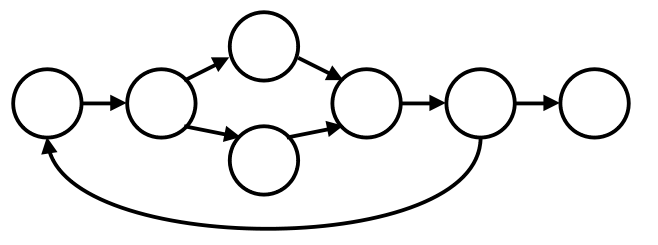
\includegraphics[width=\textwidth,height=0.45\textheight]{../Images/ExampleSlide1.png}
	\end{center}
	
\end{frame} 

% -------------- %
% -------------- %
\begin{frame}[noframenumbering]
	
	\begin{center}
		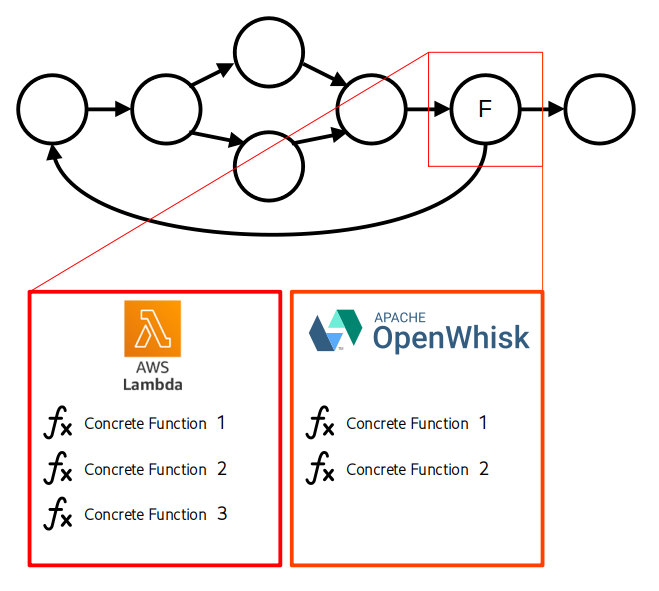
\includegraphics[width=0.9\textwidth,height=0.95\textheight]{../Images/ExampleSlide2.png}
	\end{center}
	
\end{frame} 

% -------------- %
% -------------- %
\begin{frame}[noframenumbering]
	
	\begin{center}
		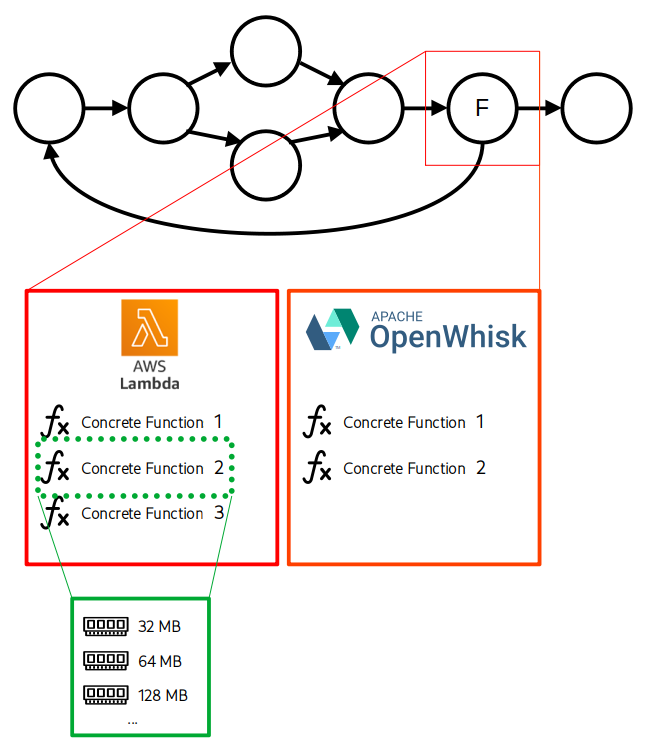
\includegraphics[width=0.8\textwidth,height=0.95\textheight]{../Images/ExampleSlide3.png}
	\end{center}
	
\end{frame} 

% -------------- %
% -------------- %
\begin{frame}
	
	\begin{center}
		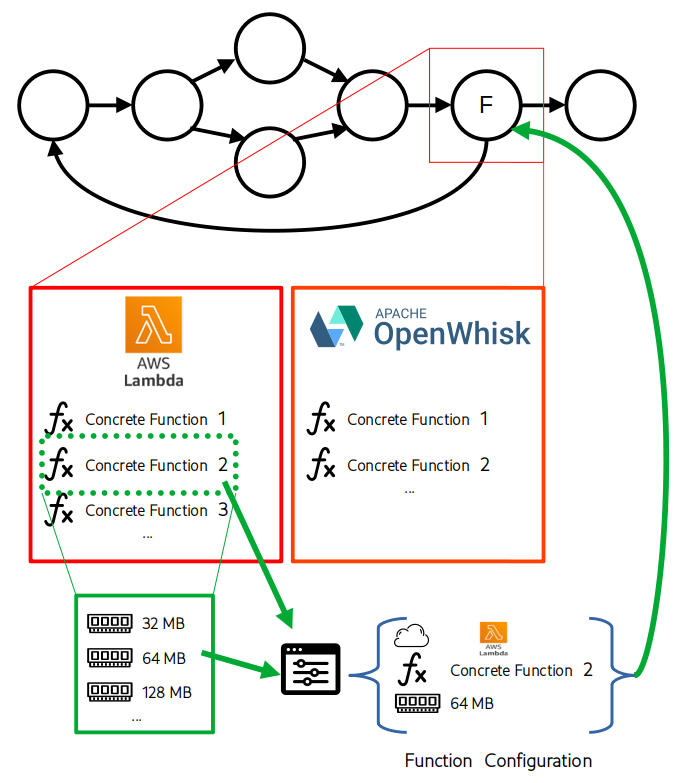
\includegraphics[width=0.8\textwidth,height=0.95\textheight]{../Images/ExampleSlide4.png}
	\end{center}
	
\end{frame} 

\begin{frame}{System Model}

\vspace{\baselineskip}
\begin{itemize}
	\item Estimations of \B{average response time} and \B{cost} under \B{any} possible configuration of all concrete functions is done using \B{exponential moving average} approach.

	\vspace{\baselineskip}
	\item An estimation of the \B{probability} according to which a request follows a cold start is required.
	\begin{itemize}
		\vspace{\baselineskip}
		\item This is done using \B{Erlang-B} formula by modeling FaaS platform providers by \B{sets} of $M/G/K(t)/K(t)$ queueing systems.
		\begin{itemize}
			\item $K(t)$: the number of function instances at time $t$.
		\end{itemize}
	\end{itemize}

	\vspace{\baselineskip}
	\item Performance estimations of the application depend on its workflow properties.
\end{itemize}

\end{frame} 
% -------------- %
% -------------- %
\begin{frame}{Optimization Problem}

\begin{itemize}
	\item To achieve our goal consisting in finding the best configuration to guarantee QoS constraints, we have to solve an \B{optimization problem}.
	\begin{itemize}
		\item It is based on \B{multi-dimensional multi-choice knapsack problem formulation} (MMKP).
	\end{itemize}
\end{itemize}

\end{frame}

% -------------- %
% -------------- %

\begin{frame}
	
\begin{figure}[h]
	\centering
	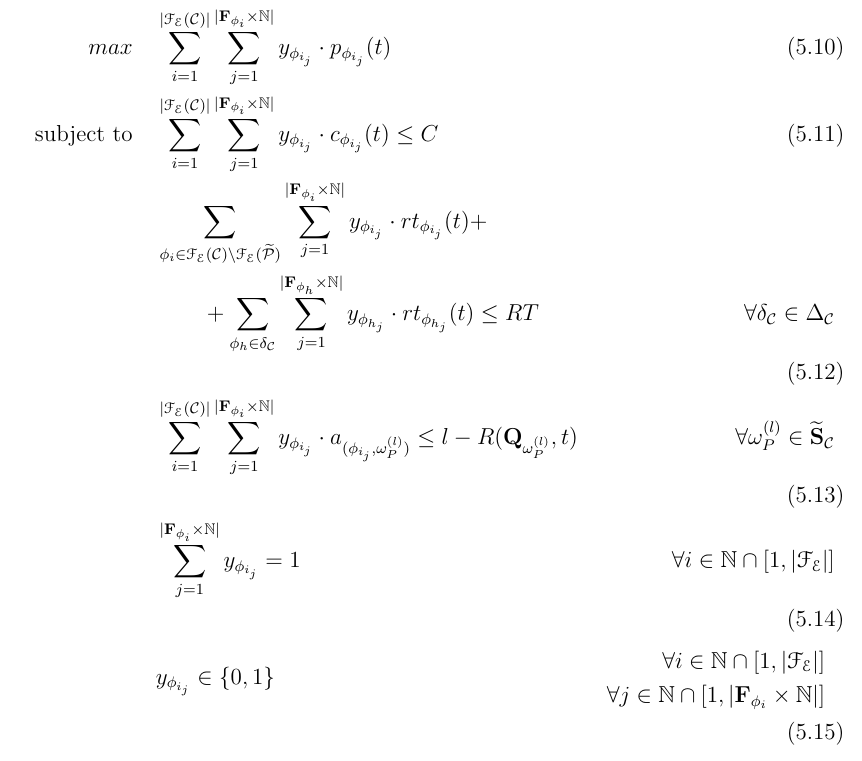
\includegraphics[width=\textwidth,height=0.8\columnwidth]{../Images/MMKPForSlide.png}
\end{figure}
	
	
\end{frame}


% -------------- %
% -------------- %
\begin{frame}[noframenumbering]
	
	\begin{figure}[h]
		\centering
		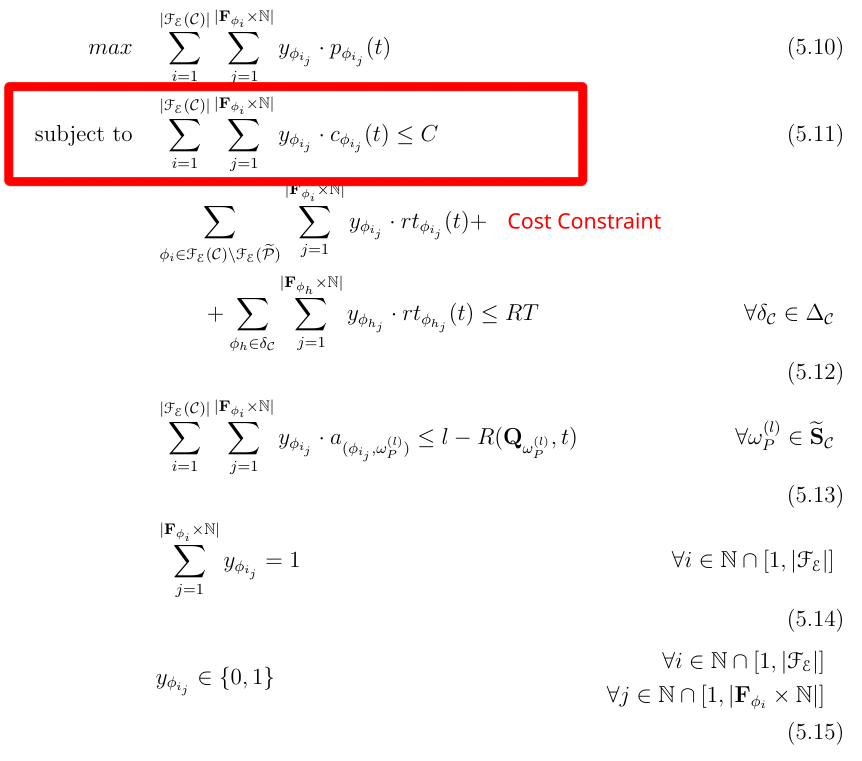
\includegraphics[width=\textwidth,height=0.8\columnwidth]{../Images/MMKPForSlide2.png}
	\end{figure}
	
	
\end{frame}



% -------------- %
% -------------- %
\begin{frame}[noframenumbering]
	
	\begin{figure}[h]
		\centering
		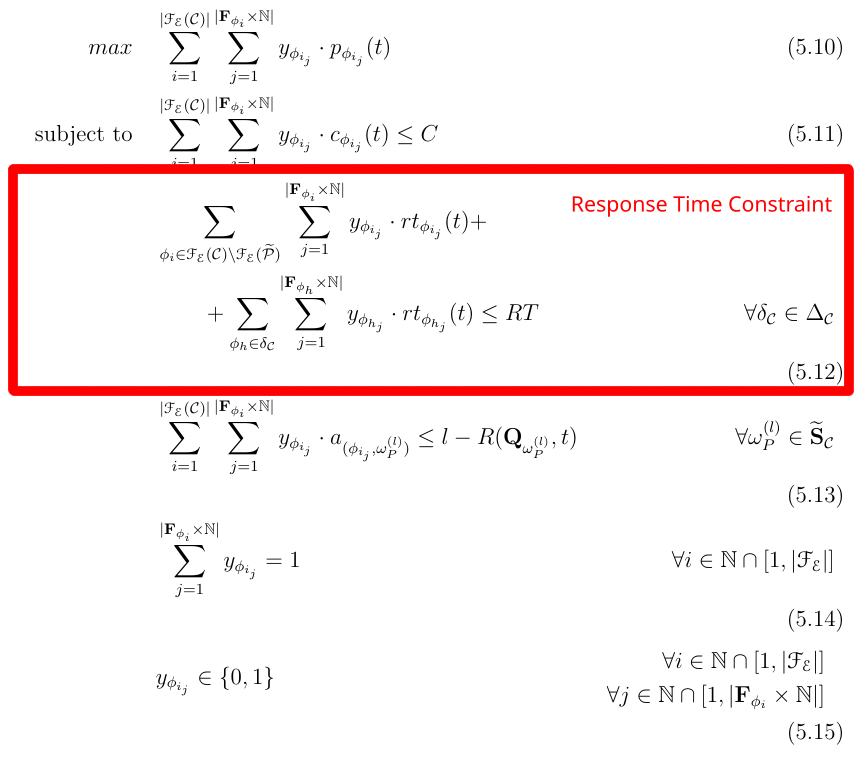
\includegraphics[width=\textwidth,height=0.8\columnwidth]{../Images/MMKPForSlide3.png}
	\end{figure}
	
	
\end{frame}



% -------------- %
% -------------- %
\begin{frame}[noframenumbering]
	
	\begin{figure}[h]
		\centering
		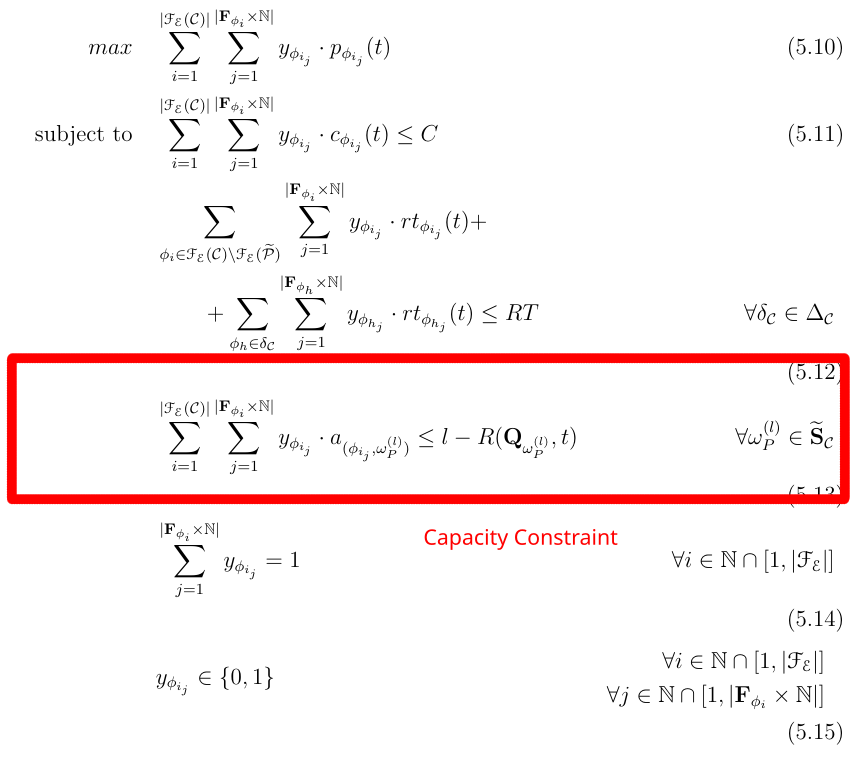
\includegraphics[width=\textwidth,height=0.8\columnwidth]{../Images/MMKPForSlide4.png}
	\end{figure}
	
	
\end{frame}



% -------------- %
% -------------- %
\begin{frame}{Heuristic Algorithm}
	
	\begin{block}{}
		\centering
		I develop a custom heuristic algorithm based on \B{ant colony optimization} (ACO).
	\end{block}
	\vspace{\baselineskip}
	\begin{itemize}
		\item It is based on a set of computational agents, called \B{artificial ants}, which \B{iteratively} construct a solution.
		
		\vspace{\baselineskip}
		
		\item At each iteration, each agent moves from a solution to another, applying a series of stochastic \B{local} decisions whose policy is based on following parameters:
		
		\begin{itemize}
			\item \B{Attractiveness}.
			\item \B{Pheromone trail}.
		\end{itemize}
		
	\end{itemize}
	
	
	
	
\end{frame}
% -------------- %
% -------------- %
\begin{frame}{Heuristic Algorithm}
	
	\begin{block}{}
		\centering
		Pheromone trails are updated during \B{every iteration}.
	\end{block}

	\begin{block}{}
		\centering
		Pheromone trails are used to decide which solutions should be preferred during \B{next iterations}.
	\end{block}

	\vspace{\baselineskip}

\end{frame}

\begin{frame}{Prototype}
	
	Main features of our software framework:
	\vspace{\baselineskip}
	\begin{itemize}
		\item \B{Client-server architecture}.
		\item \B{Cloud-native} application.
		\item Includes a set of \B{adapters} to interact with following FaaS providers:
		\begin{itemize}
			\item AWS Lambda.
			\item Apache OpenWhisk.
		\end{itemize}
		\item \B{REST} architectural style.
	\end{itemize}
	
\end{frame} 
% -------------- %
% -------------- %
\begin{frame}
	
	\begin{center}
		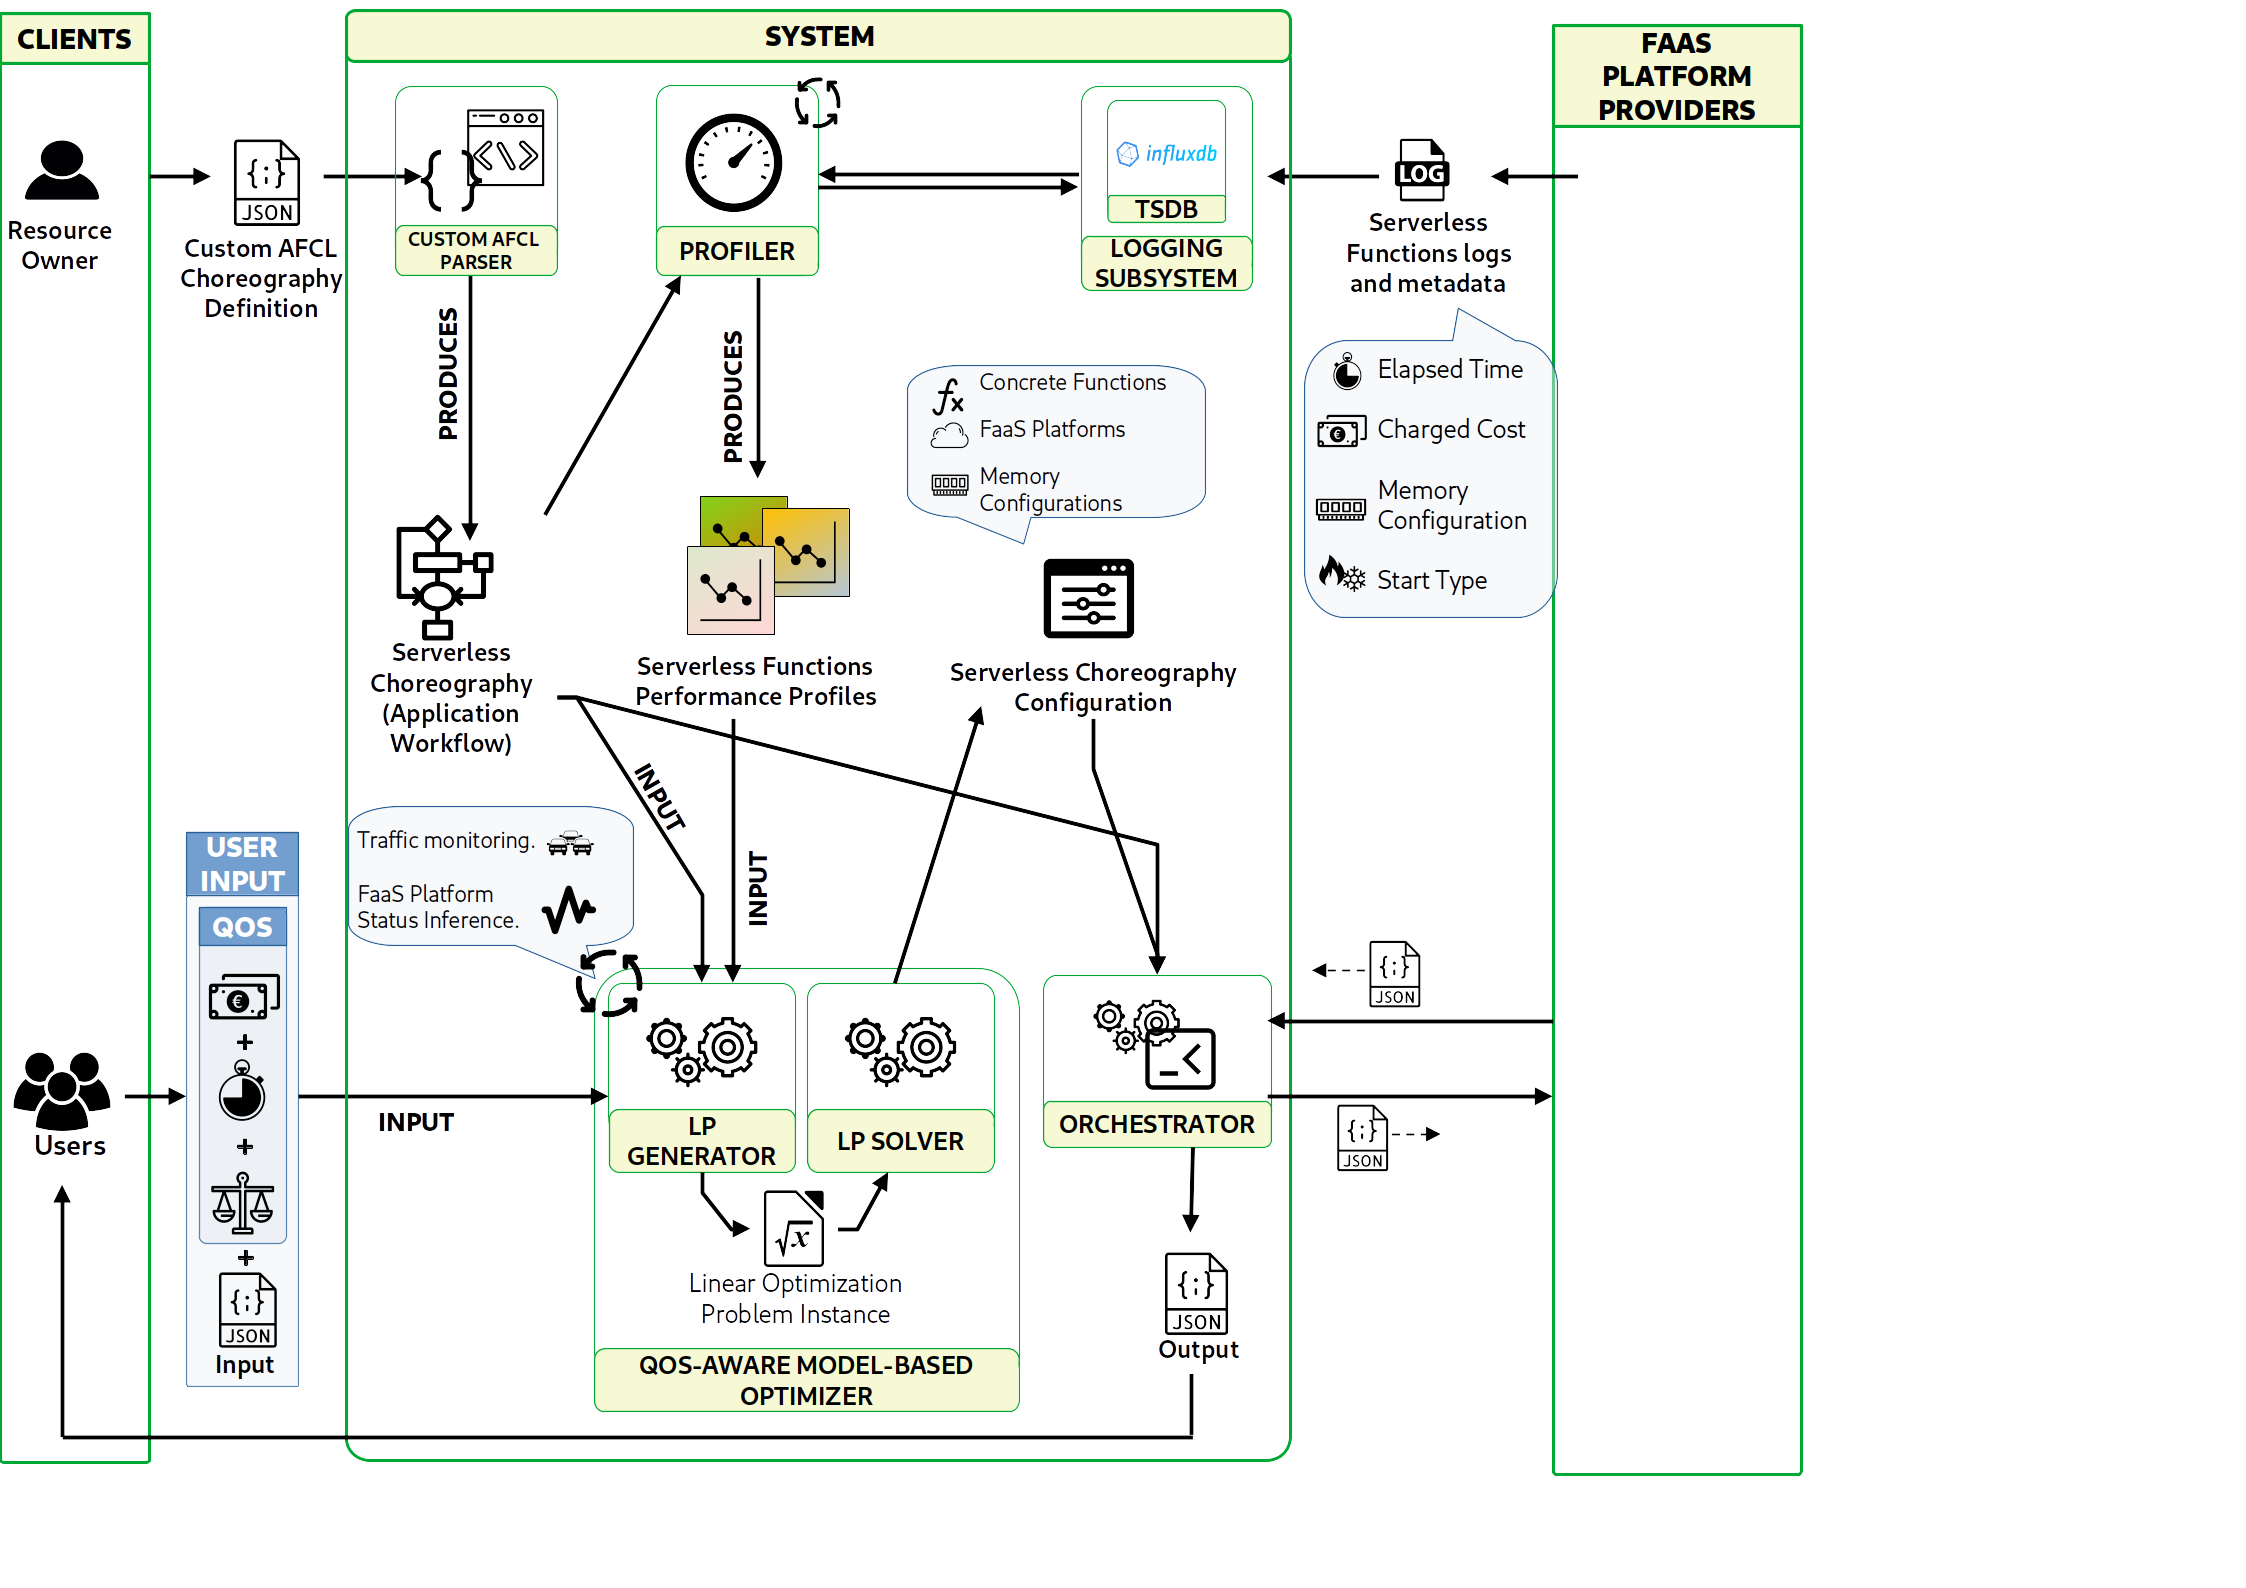
\includegraphics[width=\textwidth,height=0.95\textheight]{../Images/SystemForSlide.png}
	\end{center}
	
	
\end{frame} 

% -------------- %
% -------------- %
\begin{frame}[noframenumbering]
	
	\begin{center}
		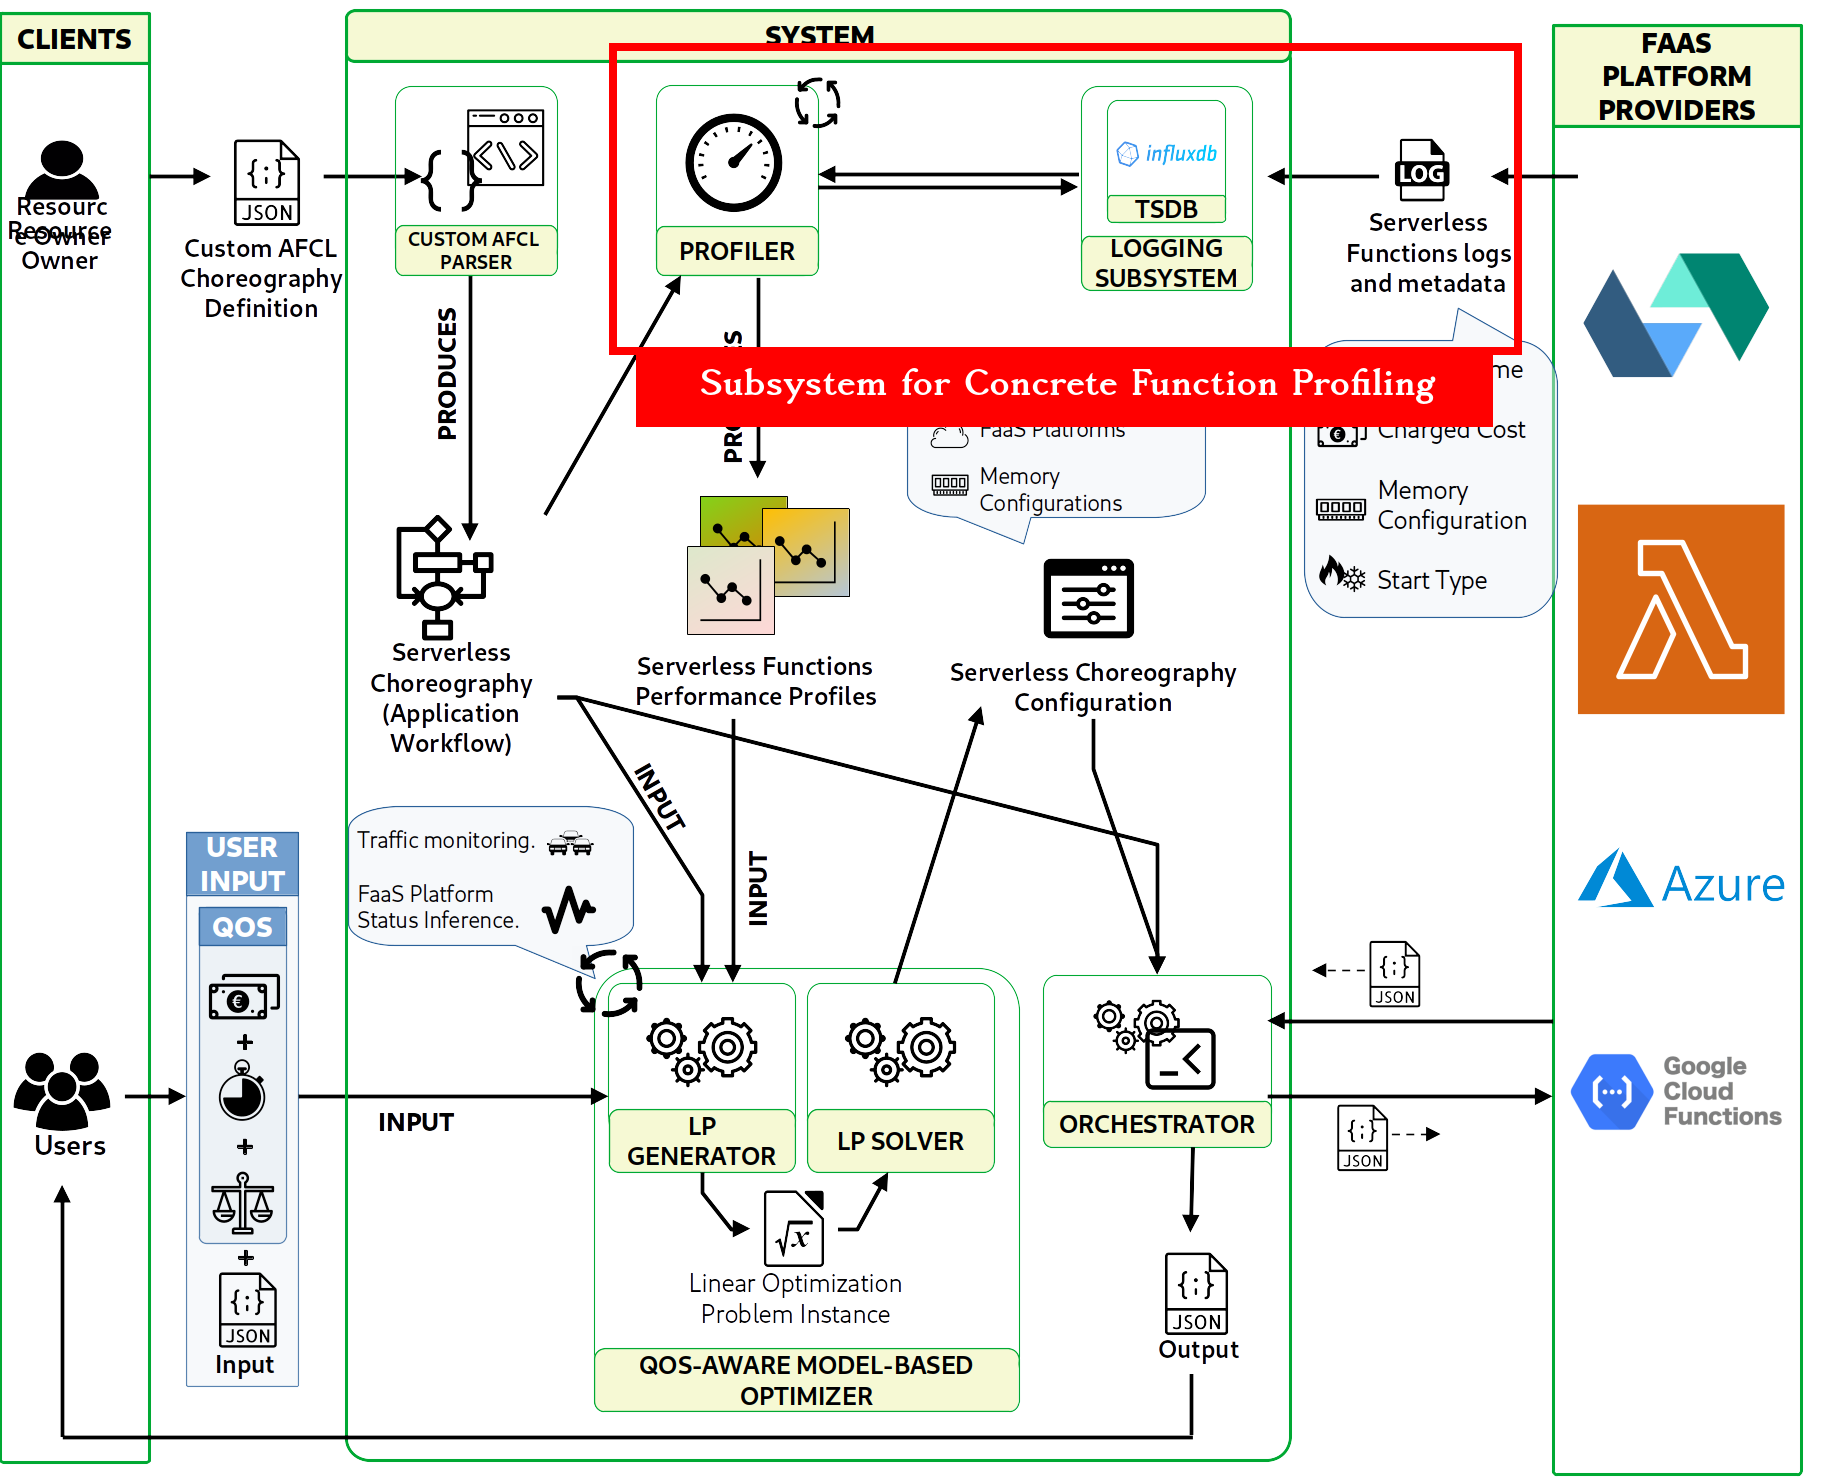
\includegraphics[width=\textwidth,height=0.95\textheight]{../Images/SystemForSlide1.png}
	\end{center}
	
	
\end{frame} 
% -------------- %
% -------------- %
\begin{frame}[noframenumbering]
	
	\begin{center}
		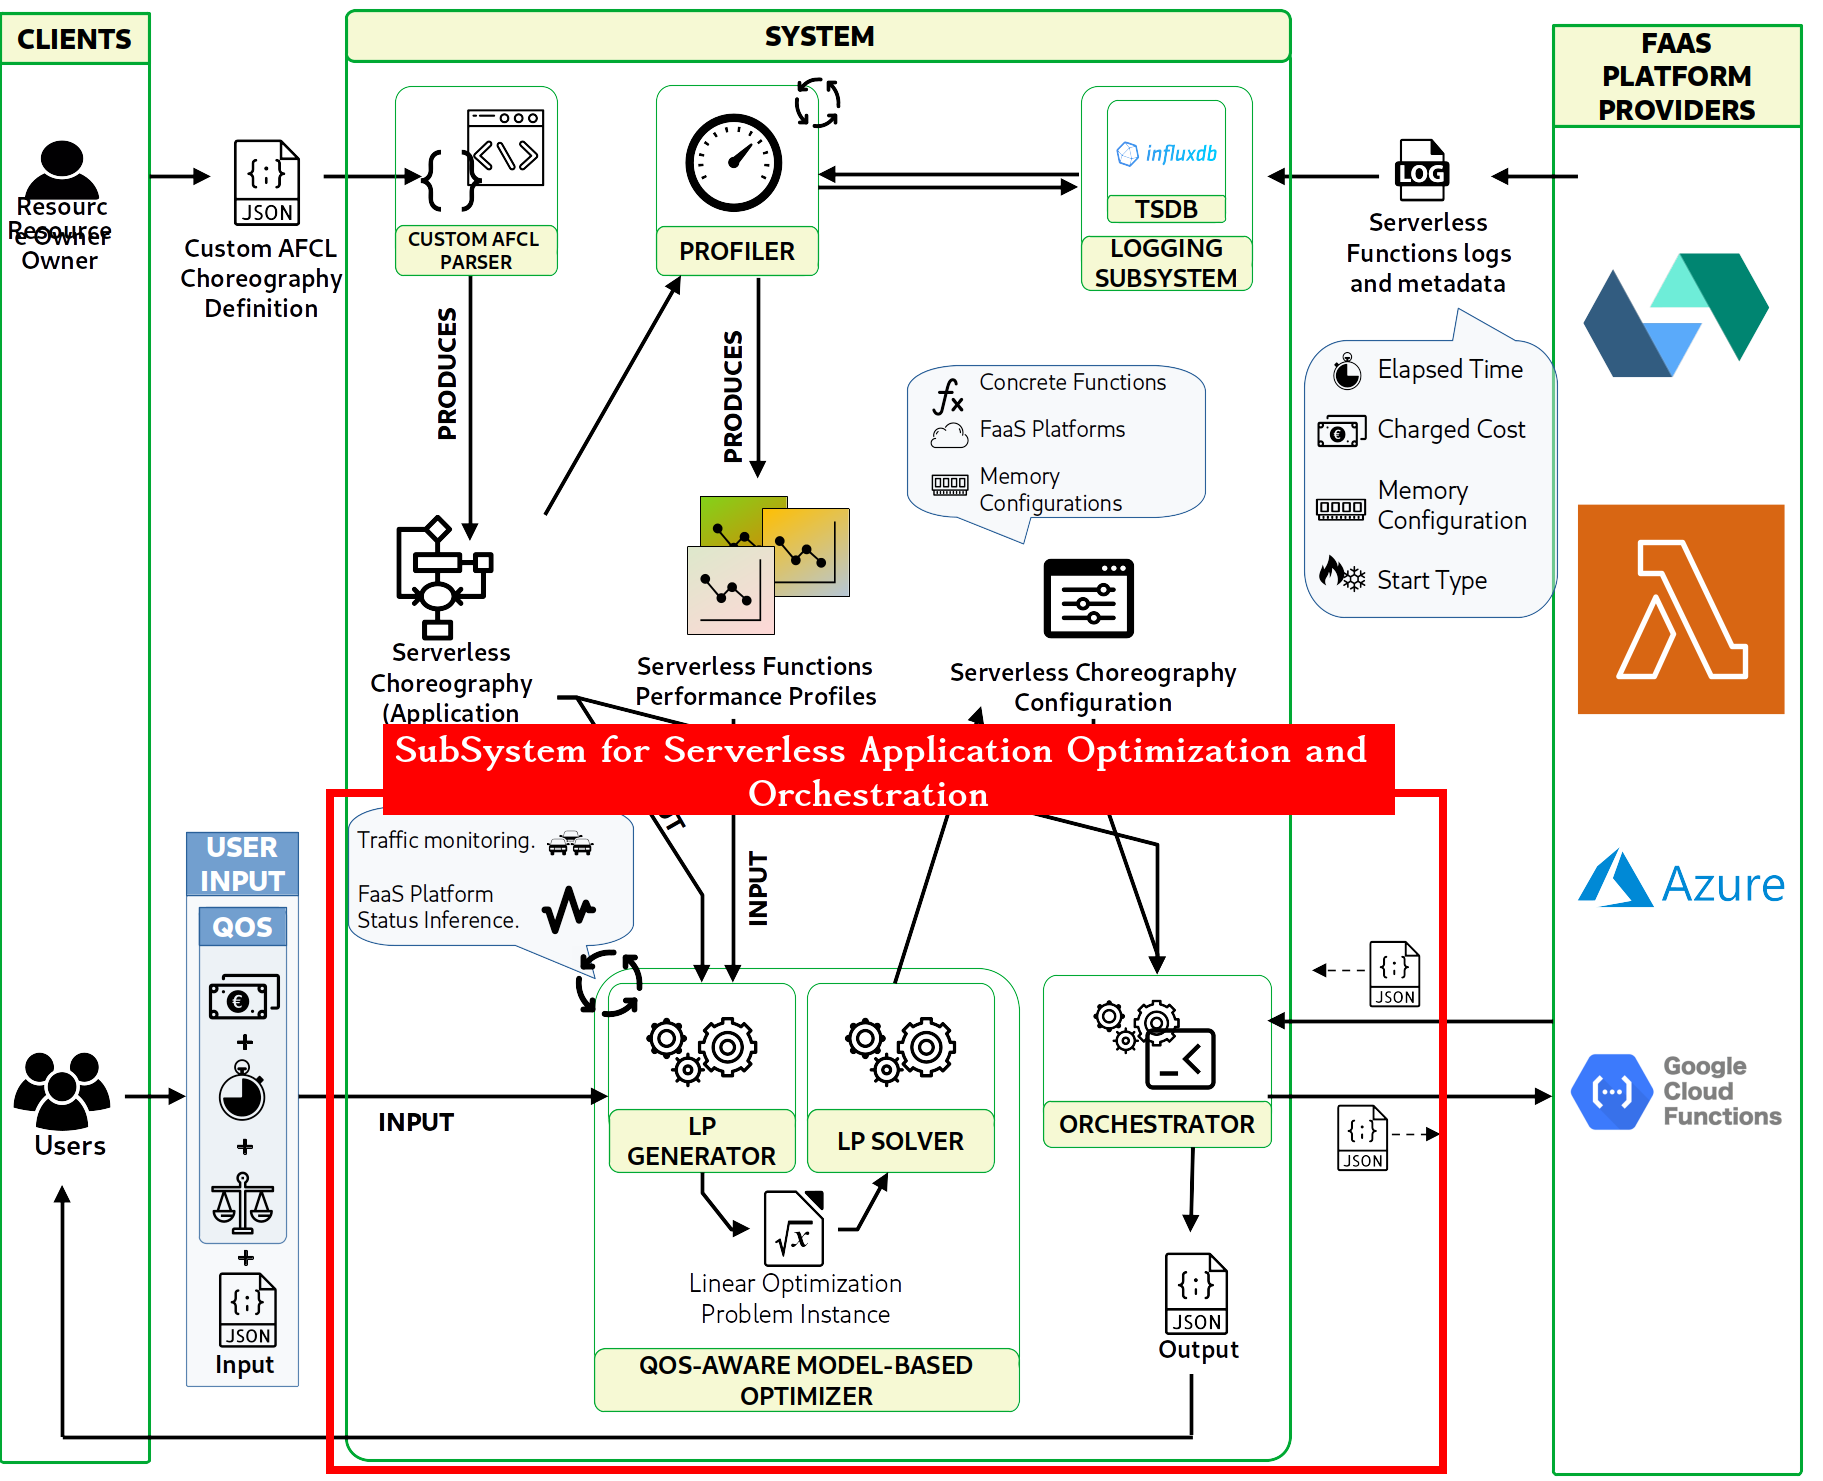
\includegraphics[width=\textwidth,height=0.95\textheight]{../Images/SystemForSlide2.png}
	\end{center}
	
	
\end{frame} 

% -------------- %
% -------------- %
\begin{frame}{Validation Test}
	
\begin{block}{}
	\centering
	We validate our model through several experiments using an image-processing serverless application.
\end{block}
	\vspace{\baselineskip}
\begin{itemize}
	\item Firstly, we check the respect of user specified QoS constraints in a static way thorough several \B{sequential invocations}.
	\vspace{\baselineskip}
	\item Then, we test the model in a dynamically way thorough \B{several concurrent and parallel invocations}. 
	\begin{itemize}
	\item That experiment aimed to \B{run out of capacity} on one FaaS provider and so force our prototype to schedule the concrete function on the other.
	\end{itemize}
\end{itemize}

\end{frame}

% -------------- %
% -------------- %

\begin{frame}{Validation Test}
	
	\begin{itemize}
		\item Application configuration produced by our system \B{before} Provider 1 runs out of capacity...
	\end{itemize}
	
	\begin{figure}[h]
		\centering
		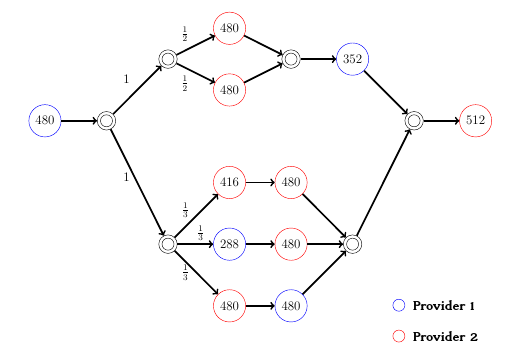
\includegraphics[width=0.8\textwidth,height=0.55\columnwidth]{../Images/EXP1ForSlide.png}
	\end{figure}
	
	
\end{frame}
% -------------- %
% -------------- %

\begin{frame}{Validation Test}
	
	\begin{itemize}
		\item ...and \B{after}, when Provider 1 runs out of capacity.
	\end{itemize}
	
	\begin{figure}[h]
		\centering
		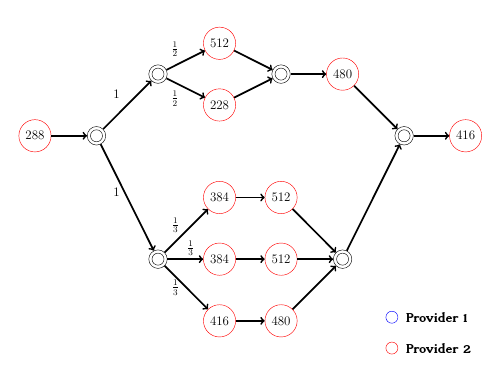
\includegraphics[width=0.8\textwidth,height=0.55\columnwidth]{../Images/EXP2ForSlide.png}
	\end{figure}
	
	
\end{frame}

% -------------- %
% -------------- %

\begin{frame}{Heuristic Algorithm Evaluation}
	
\begin{itemize}
	\item We compared \B{execution time} of our heuristic algorithm with that of optimal algorithm through several experiments.
\end{itemize}
	
	\begin{figure}[h]
		\centering
		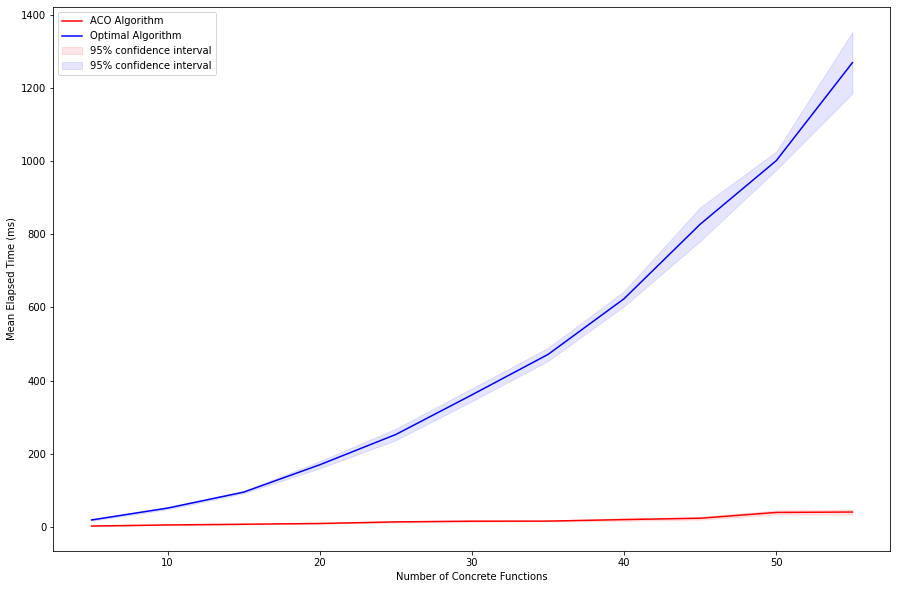
\includegraphics[width=0.8\textwidth,height=0.55\columnwidth]{../Images/ACOvsOptimalIncreasingConcrete.png}
	\end{figure}

\end{frame}

% -------------- %
% -------------- %

\begin{frame}{Heuristic Algorithm Evaluation}
	
	\begin{itemize}
		\item According to my results, \B{accuracy} is above \B{98\%}.
	\end{itemize}
	
	\begin{figure}[h]
		\centering
		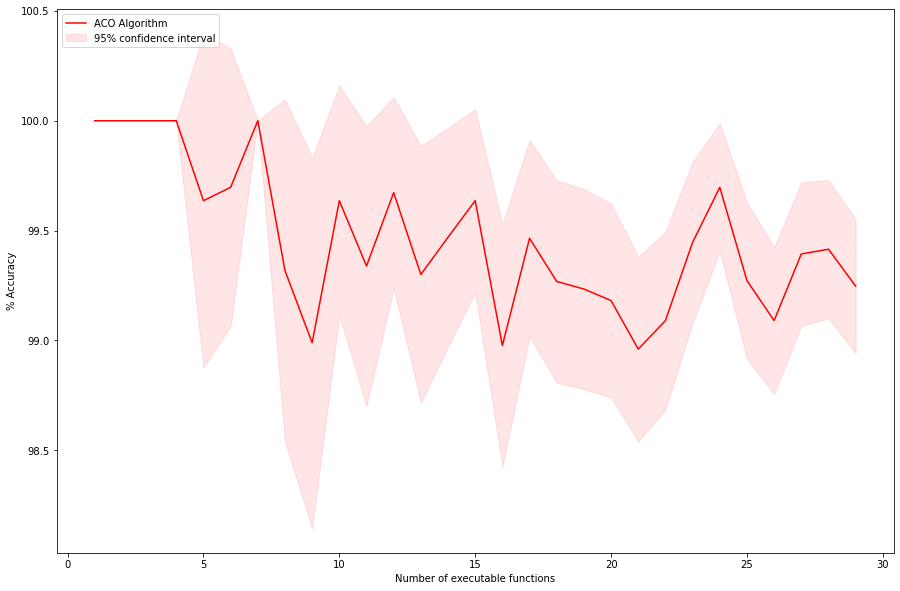
\includegraphics[width=0.8\textwidth,height=0.55\columnwidth]{../Images/ACOvsOptimalAccuracyIncreasingExecutable.png}
	\end{figure}
	
\end{frame}

% -------------- %
% -------------- %


\begin{frame}{Conclusions}

\begin{enumerate}
	
	\item I presented an analytical model to evaluate the performance of multi-provider serverless application.
	\vspace{\baselineskip}
	\item I defined an optimization problem formulation to address the problem of finding a suitable configuration in order to meet user defined QoS constraints.
	\vspace{\baselineskip}
	\item I developed a heuristic algorithm to rapidly solve it.
	\vspace{\baselineskip}
	\item I validate proposed solution through test and experimental evaluations using my prototype.	
\end{enumerate}
\end{frame}

\setbeamertemplate{background}{%
	\begin{tikzpicture}[overlay,remember picture]
		\node[scope fading=west,anchor=north west] at ([shift={(2in,-1in)}]current page.north west) {
\includegraphics[width=9cm,height=9cm]{../Images/UniLogo/TorVergataWatermark.png}};
	\end{tikzpicture}
}

\begin{frame}{{}}
	\begin{block}{}
		\centering
		Thanks for your attention!\\\B{Questions}?
	\end{block}
\end{frame} 

\end{document}
